\newcommand{\protonspeed}{$3\times10^3$ m/s}
\newcommand{\caparea}{ 4 cm$^2$}
\newcommand{\capdist}{0.5 mm}
\newcommand{\elecspeed}{$8\times10^{5}$ m/s}
\question A proton is released from rest at one end of a capacitor with area $A=$\caparea{} and begins to accelerate. At the other end of the capacitor, the velocity of the proton is \protonspeed. The plates of the capacitor are separated by a distance $d=$ \capdist.

\begin{center}
	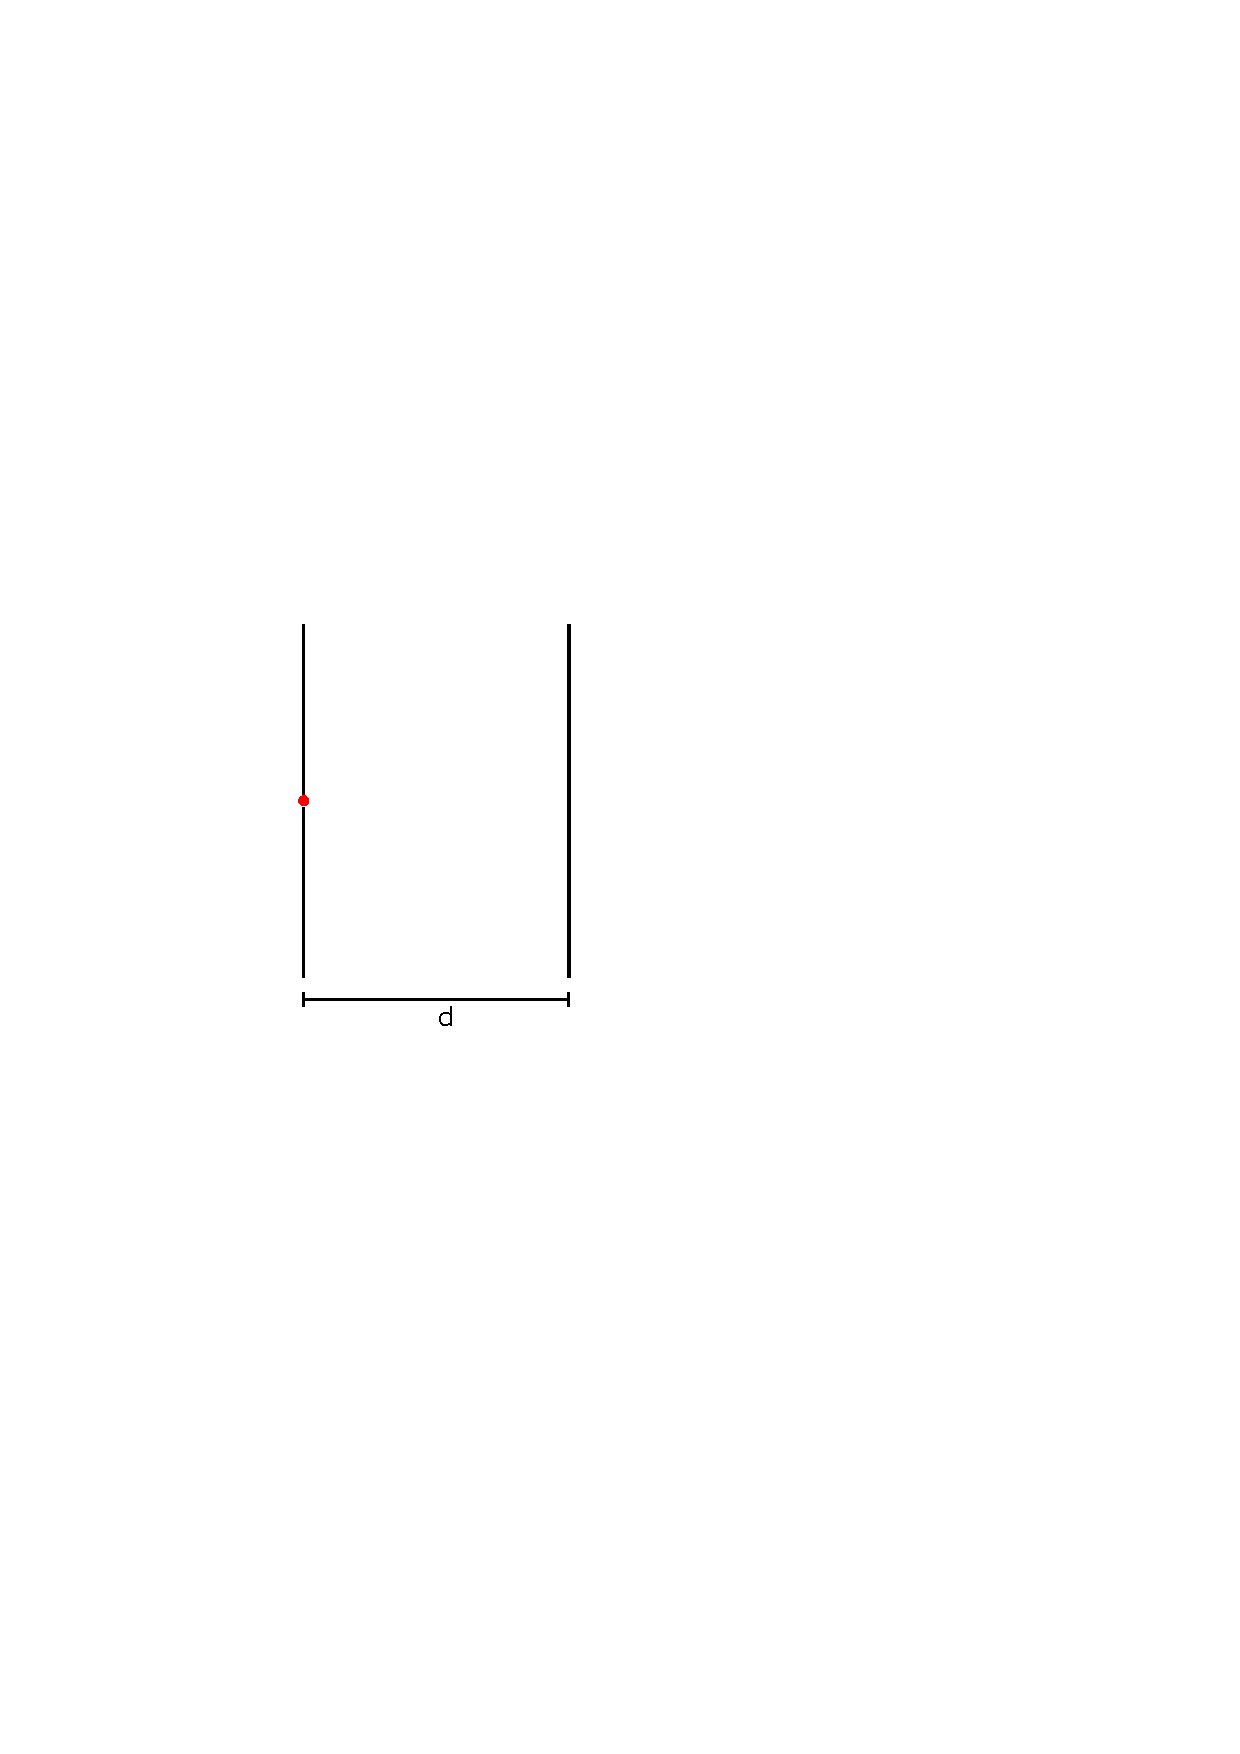
\includegraphics[width=4cm]{prob6.pdf}
\end{center}
\begin{parts}
	\part What is the potential difference $\Delta V$ of the right plate relative to the left one?
	\null\vspace{3cm}
	\part What is the magnitude and direction of the electric field inside the capacitor?
	\null\vspace{3cm}
	\part What is the charge on each capacitor plate? Which plate, right or left, carries negative charge?
	\null\vspace{3cm}
	\part An electron is shot through the tiny hole on the left side of the capacitor with an initial speed of \elecspeed{} moving from left to right. What is the velocity of the electron at the right plate?
\end{parts}